\documentclass{article}
\textheight 23.5cm \textwidth 15.8cm
%\leftskip -1cm
\topmargin -1.5cm \oddsidemargin 0.3cm \evensidemargin -0.3cm
%\documentclass[final]{siamltex}

\usepackage{verbatim}
\usepackage{fancyhdr}
\usepackage{graphicx}

%\pagestyle{fancy} \lhead{FDM Homework Template} \chead{}
%\rhead{\bfseries Yan XU}
%
%\lfoot{} \cfoot{} \rfoot{\thepage}
%\renewcommand{\headrulewidth}{0.4pt}
%\renewcommand{\footrulewidth}{0.4pt}
%
\title{FDM Homework Template}
\author{Yan XU}

\begin{document}
\maketitle

\section{Introduction}

This is where you describe the goals of this homework.

\section{Method}

Describe what you did. Did you have to innovate? Describe any
hurdles.

\section{Results}

Include and describe results obtained in this homework. You can make
a figure and print it to file, in encapsulated postscript (eps)
format. To include the eps file in your latex document as shown in
Figure \ref{figure.label}:
\begin{verbatim}
\begin{figure}[htb]
\begin{center}
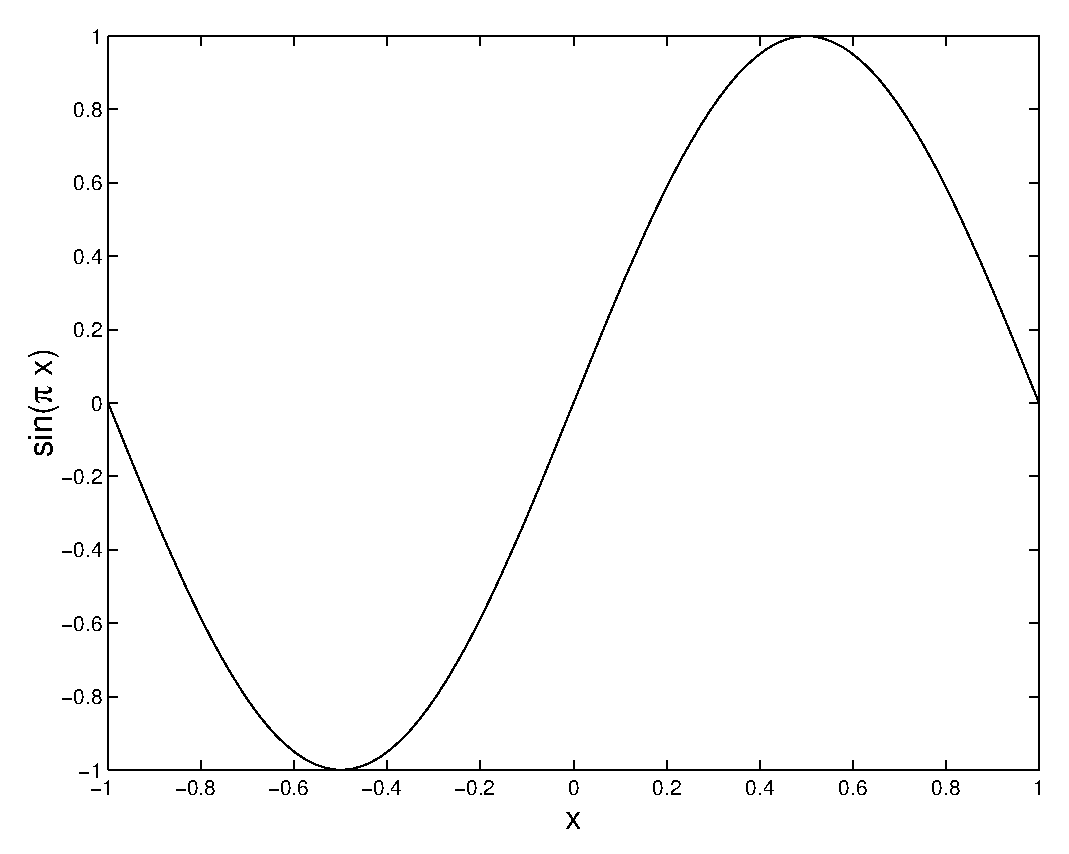
\includegraphics[width=2in]{figure.eps}
\caption{Describe the figure in this caption.} \label{figure.label}
\end{center}
\end{figure}
\end{verbatim}

\begin{figure}[htb]
\begin{center}
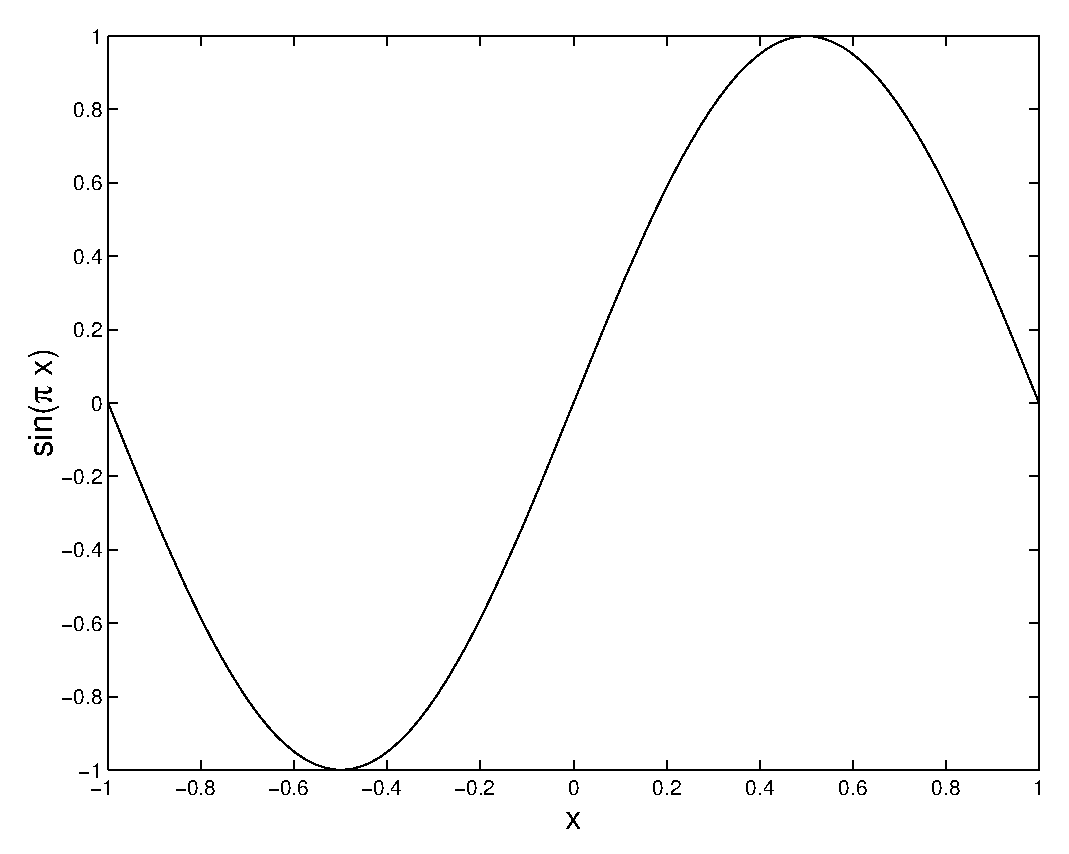
\includegraphics[width=2in]{figure.eps}
\caption{Describe the figure in this caption.} \label{figure.label}
\end{center}
\end{figure}

You can also make a table to show the accuracy results for your
method. To make a table in your latex document as shown in Table
\ref{table.label}:
\begin{verbatim}
\begin{table}[htb]
\caption{\label{table.label} Accuracy test for} \centering
\bigskip
\begin{small}
\begin{tabular}{|c|cc|cc|}
  \hline
  % after \\: \hline or \cline{col1-col2} \cline{col3-col4} ...
  n &$L^2 $ error & order &$ L^\infty$ error & order\\\hline
10&   1.16E-02  &  --   &  6.63E-02 &  -- \\
20&   3.12E-03  &  1.90 & 1.86E-02 &  1.84\\
40&   8.05E-04  &  1.95 & 4.76E-03 &  1.96 \\
80& 2.04E-04  &  1.98 & 1.19E-02 &  2.00\\\hline
\end{tabular}
\end{small}
\end{table}
\end{verbatim}

\begin{table}[htb]
\caption{\label{table.label} Accuracy test for} \centering
\bigskip
\begin{small}
\begin{tabular}{|c|cc|cc|}
  \hline
  % after \\: \hline or \cline{col1-col2} \cline{col3-col4} ...
  n &$L^2 $ error & order &$ L^\infty$ error & order\\\hline
10&   1.16E-02  &  --   &  6.63E-02 &  -- \\
20&   3.12E-03  &  1.90 & 1.86E-02 &  1.84\\
40&   8.05E-04  &  1.95 & 4.76E-03 &  1.96 \\
80& 2.04E-04  &  1.98 & 1.19E-02 &  2.00 \\\hline
\end{tabular}
\end{small}
\end{table}
\section{Discussion}

Summarize your findings and add your comments here.

\appendix
\section{Computer Code}

Here we include the computer code.

\small \hrule \verbatiminput{code.c} \hrule


\end{document}
